% =====================================================================
%  Les symptômes, un par un
% =====================================================================
\begin{frame}{Les symptômes, un par un}
  % --- moitié gauche de la capture, zoomée, sur la moitié droite de l'écran ---
  \begin{tikzpicture}[remember picture,overlay]
    % on découpe l'affichage sur la seule moitié droite de la diapositive
    \clip (current page.north) rectangle (current page.south east);
    % image affichée à 2x : ancrée par sa gauche au centre, sa moitié gauche
    % remplit alors la moitié droite de l'écran (le reste est rogné par le clip)
    \node[anchor=west,inner sep=0pt] at (current page.center)
      {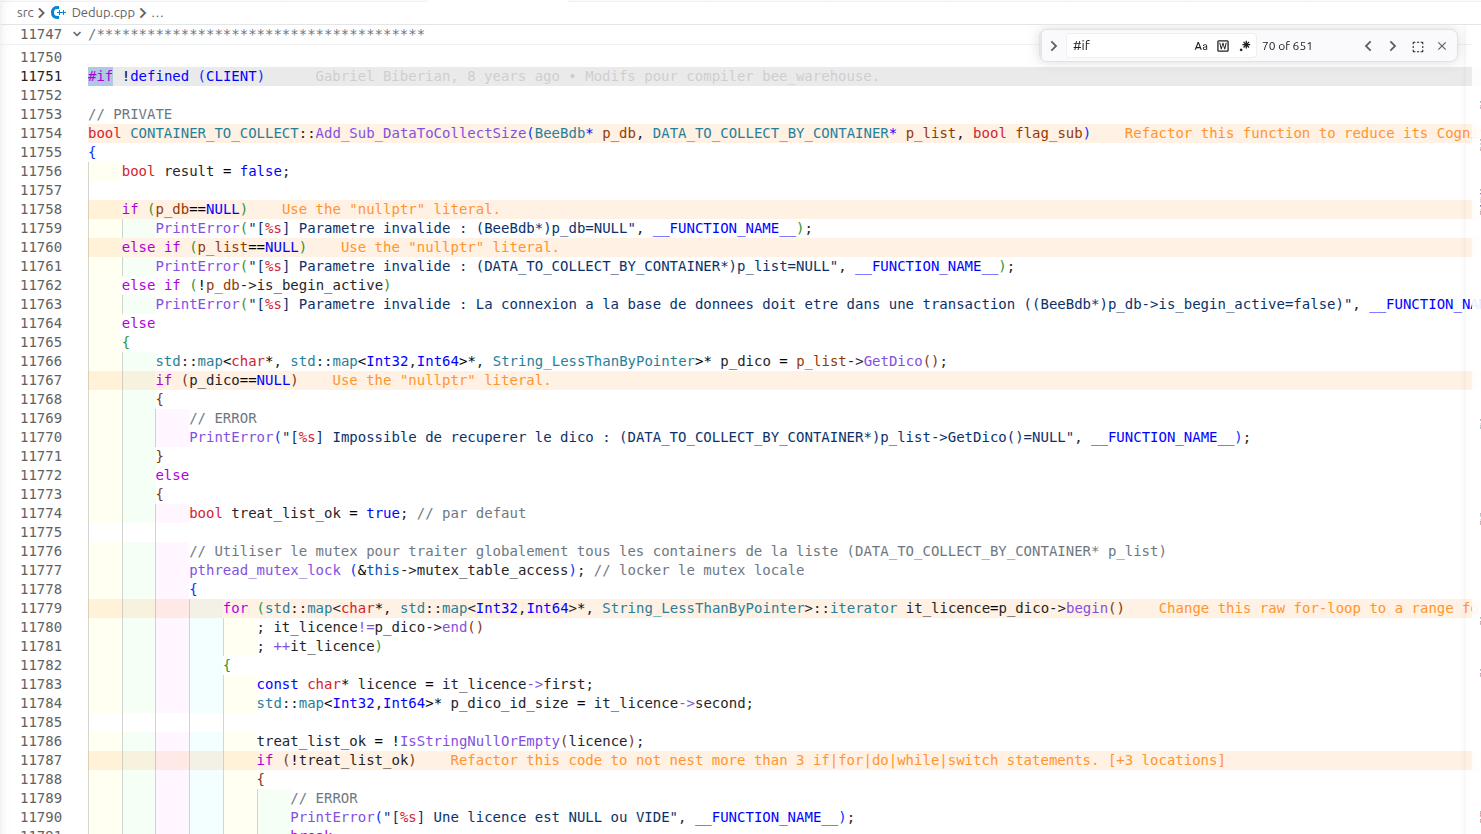
\includegraphics[width=\paperwidth]{assets/dedup-light.png}};
  \end{tikzpicture}
  \begin{columns}[c,onlytextwidth]
    \column{0.46\textwidth}
      \begin{itemize}\setlength\itemsep{0.34cm}
        \item Un \textbf{abus de directives de préprocesseur}
              (\texttt{\#ifdef}) pour gérer les cas de compilation.
        \item Des \textbf{fonctions interminables} et une maîtrise
              approximative du C++ (jusqu'à des tests
              \texttt{this == nullptr}, un \emph{undefined behavior}).
        \item Une \textbf{absence totale de tests} : aucun filet de sécurité.
        \item Un \texttt{main.h} qui \textbf{inclut tout le projet} : un
              couplage massif.
      \end{itemize}
    \column{0.50\textwidth}\mbox{}
  \end{columns}
\end{frame}
